\documentclass[10pt,a4paper,twoside]{article}
\usepackage{graphicx}
\usepackage{floatflt}

%%%%%%%%%%%%%%%%%%%%%%%%%%%%%%%%%%%%%%%%%%%%%%%%%%%%%%%%%%%%%%%%%%%%%%%%%%%%%%%
%%%%%%%%%%%%%%%%%%%%%%%%%%%%%%%%%%%%%%%%%%%%%%%%%%%%%%%%%%%%%%%%%%%%%%%%%%%%%%%
%% Some previous definintions
\setlength{\voffset}{-1in}
\setlength{\hoffset}{-1in}
\setlength{\oddsidemargin}{3cm}
\setlength{\evensidemargin}{2cm}
\setlength{\textheight}{25cm}
\setlength{\textwidth}{16cm}

\newcommand{\octopus}{{\tt octopus}\ }

\newcounter{inputfiles}
\newcounter{outputfiles}
\newsavebox{\captiontext}
\newsavebox{\verbatimtext}
\newsavebox{\labeltext}

\newenvironment{mylist}
{
\begin{list}{$\aleph$}
{
\setlength{\parskip}{0pt}
\setlength{\topsep}{0pt}
\setlength{\partopsep}{0pt}
\setlength{\itemsep}{0pt}
\setlength{\parsep}{0pt}
}
}
{
\end{list}
}


\newcounter{exercises}
\newenvironment{exerciselist}
{
\refstepcounter{exercises}

{\bf Exercise~\arabic{exercises}}:
\begin{list}{$\dagger$}
{
\setlength{\parskip}{0pt}
\setlength{\topsep}{0pt}
\setlength{\partopsep}{0pt}
\setlength{\itemsep}{0pt}
\setlength{\parsep}{0pt}
}
}
{
\end{list}
}



\newenvironment{sampleinput}[2]
{
\sbox{\captiontext}{#1}
\begin{lrbox}{\verbatimtext}
\refstepcounter{inputfiles}
\label{#2}
\begin{minipage}{0.9\textwidth}
\footnotesize
}
{
\end{minipage}
\end{lrbox}
\begin{center}
\noindent\framebox{\usebox{\verbatimtext}}
\end{center}
\begin{center}
Input File \arabic{inputfiles}: {\usebox{\captiontext}}
\end{center}
}

\newenvironment{sampleinputcont}[1]
{
\sbox{\captiontext}{#1}
\begin{lrbox}{\verbatimtext}
\begin{minipage}{0.9\textwidth}
\footnotesize
}
{
\end{minipage}
\end{lrbox}
\begin{center}
\noindent\framebox{\usebox{\verbatimtext}}
\end{center}
\begin{center}
Input File \arabic{inputfiles} (continued): {\usebox{\captiontext}}
\end{center}
}

\newenvironment{sampleoutput}[2]
{
\sbox{\captiontext}{#1}
\begin{lrbox}{\verbatimtext}
\refstepcounter{outputfiles}
\label{#2}
\begin{minipage}{0.9\textwidth}
\footnotesize
}
{
\end{minipage}
\end{lrbox}
\begin{center}
\noindent\framebox{\usebox{\verbatimtext}}
\end{center}
\begin{center}
Output box \arabic{outputfiles}: {\usebox{\captiontext}}
\end{center}
}

\newenvironment{sampleoutputcont}[1]
{
\sbox{\captiontext}{#1}
\begin{lrbox}{\verbatimtext}
\begin{minipage}{0.9\textwidth}
\footnotesize
}
{
\end{minipage}
\end{lrbox}
\begin{center}
\noindent\framebox{\usebox{\verbatimtext}}
\end{center}
\begin{center}
Output box \arabic{outputfiles} (continued): {\usebox{\captiontext}}
\end{center}
}

\setlength{\parskip}{0.0ex plus0.0ex minus0.0ex}
%%%%%%%%%%%%%%%%%%%%%%%%%%%%%%%%%%%%%%%%%%%%%%%%%%%%%%%%%%%%%%%%%%%%%%%%%%%%%%%
%%%%%%%%%%%%%%%%%%%%%%%%%%%%%%%%%%%%%%%%%%%%%%%%%%%%%%%%%%%%%%%%%%%%%%%%%%%%%%%








%%%%%%%%%%%%%%%%%%%%%%%%%%%%%%%%%%%%%%%%%%%%%%%%%%%%%%%%%%%%%%%%%%%%%%%%%%%%%%%
%%%%%%%%%%%%%%%%%%%%%%%%%%%%%%%%%%%%%%%%%%%%%%%%%%%%%%%%%%%%%%%%%%%%%%%%%%%%%%%
\begin{document}

\title{A short tutorial on the \octopus code}
\author{[Tutorial based on the 1.4 version]}
\maketitle


\begin{center}
\begin{minipage}{0.8\textwidth}
\small
This document is an introduction to the usage of the
\octopus code. It presents a series of simple
input files, which exemplify the most important
possible uses of the code, along with the expected
output files. Both input variables and output
files are explained, although there is no attempt
to give a comprehensive review of all possible variables
-- and the values that these may take --
or running possibilities; it is the \octopus manual
which attempts to do that.
\end{minipage}
\end{center}

\tableofcontents


\section{A simple example: The Nitrogen atom}

As a first warm-up run, we will obtain the ground-state
of an atomic system. We will give a rather detailed description
of the input and output files for this first example.

\subsection{The input file}

The sample input file \ref{input:nitrogen_atom_gs} 
permits to obtain the ground state
of the Nitrogen atom, within the LDA approximation, in a closed-shell
(unpolarized configuration). It will permit us to describe
some of the most important input variables:
\begin{sampleinput}{The Nitrogen atom}{input:nitrogen_atom_gs}
\begin{verbatim}
CalculationMode = gs_start

units = 'eVA'

Nitrogen_mass = 14.0
Nitrogen_z = 7

%Species
'N' | Nitrogen_mass | Nitrogen_z | 'tm2' | 1 | 0
%

XYZCoordinates = 'N.xyz'

ExtraStates = 1
%Occupations
2 | 1 | 1 | 1
%

BoxShape = sphere
radius = 5.0
spacing = 0.18

LocalPotentialSpace = real_space

TypeOfMixing = broyden
\end{verbatim}
%\label{input:nitrogen_atom_gs} 
\end{sampleinput}
\begin{mylist}
\item {\tt CalculationMode = gs\_start}\\
This variable defines the run mode -- please consult the manual for the
full list of the possible run modes. In this case we set it to {\tt gs\_start},
which instructs the code to start a ground-state calculation.

Note that {\tt gs\_start} is nothing else than a mnemonic for
the value {\tt 1}, which is the one that determines the run mode. I.e. if
you write {\tt CalculationMode = 1}, you get the same behavior. Most
variables whose list of accepted values are numeric have this kind of mnemonic
helps -- the full list of equivalence is given in the {\tt SHARE/octopus/variables}\footnote{
The octopus code is installed, as described in the manual under some directory
which hereafter we will call {\tt PREFIX}. The executables are then placed
in {\tt PREFIX}/bin, and a directory called {\tt PREFIX/share/octopus} will be created.
We will call {\tt SHARE = PREFIX/share}.}
file. It is better to use the mnemonic equivalent rather than the numerical
value directly.
\item {\tt units = 'eVA'}\\
Two different units systems may be used both for input and output: the usual
atomic units (which is the default, and the one used internally in the code);
and the system in which the atomic unit of length is substituted by the Angstrom, and
the atomic unit of energy is substituted by the electronvolt. This is the case in
this input file.
\item The following two entries in the input file are not \octopus variables,
but rather illustrate the possibility of writing ``user defined'' values and
expressions. In this case, we define the atomic number of Nitrogen
({\tt Nitrogen\_mass = 14.0}), and its
mass ({\tt Nitrogen\_z = 7}) (note that in this case, as an exception, the value is expected to be in
the so called ``atomic units of mass'', rather than in ``atomic units'' or
in the other {\tt 'eVA'} system). These definitions may be used elsewhere in the input file,
as we shall see in the following entry.
\item The next entry is not just the definition of a variable, but rather
of a full set of them -- a ``block'' of variables. The beginning of a block
is marked by the {\tt \%identifier} line, and ended by a {\tt \%} line.
The {\tt identifier} in this case is {\tt Species}. This block should contain
the list of species that are present in the system to be studied; in this
simple example, just Nitrogen. This is why this block only has one line, 
whose first entry is precisely the string {\tt 'N'} for Nitrogen. Note that each entry
is separated by a {\tt |} separator (a {\sc tab} could be used as well).

The following entry of the line should contain the mass of the species, and in 
this case we have made use of the user defined variable {\tt Nitrogen\_mass} that
we have previously defined. It is also the case of the third entry, which contains
the atomic number.

The fourth entry is the {\tt 'tm2'} string. It instructs the {\tt octopus} to use
a Troullier-Martins pseudopotential for this Nitrogen atom. In practice, this means
that the {\tt octopus} will try to find a {\tt N.ascii} file either in the
working directory (from where the {\tt octopus} was launched) or in
the directory {\tt SHARE/octopus/PP/TM2} directory.

The following two entries require some knowledge of what nonlocal pseudopotentials
are, and how Troullier-Martins pseudopotentials are constructed. We do not describe them
here; suffice it to say that the two values entered here are perfectly reasonable for Nitrogen.

[Once again, we refer the reader to the \octopus manual for a more complete
description of the possiblities of the {\tt\%Species} block]

\item {\tt XYZCoordinates = 'N.xyz'}\\
The geometry of the molecule (in this case, a single atom in the grid origin) is
described in this case in a file with the well known {\tt XYZ} format.
The file for this outrageously simple case is given in the box corresponding to the
Input file~\ref{input:N.xyz}.

\item {\tt ExtraStates = 1}\\
By default, the \octopus performs spin-unpolarizad calculation (restricted closed-shell,
in Hartree-Fock terminology). It then places two electrons per orbital. The number
of orbitals, or Kohn-Sham states, is then calculated by counting the number of
valence electrons present in the system, and dividing by two. In this case, since we have five
valence electrons, the code would use three orbitals. However, we know beforehand
that the HOMO orbital has a three-fold degeneracy, and as a consequence we need to put
each one of the three $p$ electrons in a different orbital. We therefore need
one more orbital, and this is the request of this entry in the input file.

\item {\tt \%Occupations} block.\\
In principle, the occupations of the Kohn-Sham orbitals are automatically decided
by the code, filling the lowest-energy orbitals. However, if we have degeneracies
in the LUMO as it is the case, the user may want to accomodate the electrons
in a certain predefined way. In this example, th obvious way to fill the orbitals
of the Nitrogen atom is to put two electrons in the first and deepest orbital
(the $s$ orbital), and then one electron on each of the second, third and fourth
orbitals (the $p$ orbitals, which should be degenerate).

\item {\tt BoxShape = sphere}\\
This is the choice of the shape of the simulation box, which in this case is set 
to be a sphere (other possible choices are {\tt cylinder}, or {\tt parallelepiped}).

\item {\tt radius = 5.0}\\
The radius of the sphere, obviously. As the requested unit system was {\tt 'eVA'},
this means 5\AA.

\item {\tt spacing = 0.18}\\
As you should know, \octopus works in a real space regular cubic mesh.
This is the spacing between points, a key numerical parameter, in some
ways equivalent to the energy cutoff in plane wave calculations.

\item {\tt LocalPotentialSpace = real\_space}\\
By default, this version of \octopus stores the local part of the pseudopotential in 
Fourier space, and every time that the geometry is modified, it is transformed to 
real space, where it is applied. The reason for doing this is that it is a way to
minimize the so-called eggbox effect, which we will discuss later. However, this has
a serious impact on the performance, and on the memory usage. On top of this, it is completely
useless if the atoms are not allowed to move. We have thus included this
variable here to force genuine real space local potentials.
[Incidentally, in the next version of \octopus this variable is gone altogether,
in favor of a better scheme].

\item {\tt TypeOfMixing = broyden}\\
If you know something about the Kohn-Sham problem, you know that it is a non-linear
problem, and that it must be solved via a self-consistent procedure. This involves
an iterative scheme in which a series of approximative electronic densities
is constructed, hopefully convergent (in rather mysterious ways) to the exact solution
density. At each step, an ``input'' density is needed to feed the Hamiltonian,
and this ``input'' density is constructed from the densities of previous steps
by making use of some ``mixing'' procedure. By default, the so-called {\tt linear}
scheme is used, which is safe, but extremely slow. A more sophisticated scheme
is the so-called {\tt broyden} scheme, chosen for this input file.

[Once again, and this is the last time, we remind the reader that this tutorial
only attempts to be a first introduction to the code, and not a comprehensive
description of all algorithms and input variables. The manual is a little bit
more comprehensive, and the \octopus papers contain more on algorithmic details.]

\end{mylist}




\begin{sampleinput}{The {\tt N.xyz} file}{input:N.xyz}
\begin{verbatim}
1

N 0 0 0
\end{verbatim}
\end{sampleinput}

\subsection{Results: The output files}

Once constructed the input file, you may launch the \octopus on it. The
output boxes \ref{output:nitrogen_first}, \ref{output:nitrogen_second}
and \ref{output:nitrogen_last} contain some portions of what is written
to standard output.

In the first output box, you may see the first information that you will get.
First, a reminder of the version that is being used (1.4, in this case), and when it was built.
Then, the code informs on which machine it is running, and under which
operating system (in this case, my desktop, called {\tt g32}, running {\tt Linux}.
Next, it tells when the \octopus was launched.

Since there is the option of running with models potentials in one and two dimensions,
then the code informs us that {\tt Octopus will run in 3 dimension(s)}.
The system is not supposed to be periodic in any of the three dimensions
(in fact, this version of the code does not allow any dimension to be periodic),
and zero boundary conditions are considered outside the simulating box.

Next the code searches the needed psedopotential files, and informs
the user about its success or failure. In this case, only the {\tt N.ascii} file
is required and processed.

The following step is the construction of the mesh. As requested in the input file,
a sphere of 5\AA~of radius is used, which contains a cubic regular real-space grid
with 0.18\AA~of spacing. This implies 89727 points ({\tt inner mesh =  89727}).
For the sake of comparison with plane-wave based codes, this is more or less equivalent
to a plane wave calculation that imposes a cutoff of 1160.595~eV (except that in this
case there is no artificial periodic repetition of the system).

The next line [{\tt Info: Derivatives calculated in real-space}] informs us that the
derivatives operators are calculated in real space, i.e. by making use of
finite difference schemes. This is, of course, the default and recommended choice
for a real space code (however, one could perform this operations in Fourier space).
Also, and as requested in the input file, the code informs us that
the local potential action is operated in real space.

The next four lines are concerned with the Poisson solver -- since no input variable
regarding this issue was given, the code makes use of the default option: a FFT-based
solver that imposes of a spherical cutoff on the Hartree potential. 
This option is usually good enough for
normal molecules.

After the line {\tt Info: Exchange and correlation}, you can see the default options
for these terms of the Hamiltonian: the local density approximation (LDA) for
both exchange and correlation (the non-relativistic expression for the former case,
and the parameterization of Perdew and Zunger for the latter).

The code then tells us that it is allocating memory for the
wavefunctions ({\tt Allocating rpsi}), and that it is putting
random functions in it. After that, it substitutes these random functions
by atomic orbitals (calculated previously when the pseudopotentials were constructed).
It then integrates the total charge contained in these atomic orbitals. It should
integrate to the number of electrons; anyerror should be ascribed to a too
small box, or too big grid spacing.\footnote{
Except in the case of the Troullier-Martins Nitrogen pseudopotential distributed
with octopus (exactly the one that we are using for this example), which for some
odd unimportant reason lacks 0.2 electrons per atom. This is way the number
given is approx. 4.8 electrons.
}
In any case, right afterwards, these starting orbitals are normalized to give
exactly the number of valence electrons:
{\tt Info: Renormalized total charge =      5.000000}.
\begin{sampleoutput}{The Nitrogen atom: first part of the output}{output:nitrogen_first}
\begin{verbatim}
                     Running octopus, version 1.4
             (build time - Mon Jan 24 16:22:00 CET 2005)

                The octopus is swimming in g32 (Linux)
Info: Calculation started on 2005/01/26 at 19:01:22
Info: Octopus will run in 3 dimension(s)
Info: Octopus will treat system as periodic in 0 dimension(s)
Info: Boundary conditions: zero wave-functions
Info: Reading pseudopotential from file:
      '/home/alberto/software/octopus/1.4a/share/octopus/PP/TM2/N.ascii'
      Calculating atomic pseudo-eigenfunctions for specie N ....
      Done.
Info: l =  0 component used as local potential
  Type = sphere
  Radius  [A] =   5.000
  Spacing [A] = ( 0.180, 0.180, 0.180)    volume/point [A^3] =  0.00583
  # inner mesh =  89727
  Grid Cutoff [eV] =  1160.595
Info: Derivatives calculated in real-space
Info: Local Potential in Real Space.
Info: Using FFTs with spherical cutoff
      to solve Poisson equation
Info: FFT allocated with size ( 125, 125, 125) in slot  1
Info: Poisson Cutoff Radius [A] =    11.250000
Info: Exchange and correlation
      Exchange    : LDA  - non-relat.
      Correlation : LDA  - PZ81
Info: Allocating rpsi.
Info: Random generating starting wavefunctions.
Info: Unnormalized total charge =      4.792825
Info: Renormalized total charge =      5.000000
Info: Setting up Hamiltonian.
\end{verbatim}
\end{sampleoutput}
Let us know take a look at the Output box~\ref{output:nitrogen_second},
to see how the code pursues its calculation. The first step is to obtain a reasonably
good starting density and KS orbitals to feed in the self consistent (SCF) procedure.
For this purpose, \octopus performs an initial calculation restricted to the basis
set of atomic orbitals (Linear Combination of Atomic Orbitals, LCAO). The resulting
eigenvalues of this calculations are cast to standard output.

Following, the SCF procedure starts ({\tt Info: SCF using real wavefunctions}).
[Complex wave-functions should be used -- by making use of the {\tt octopus\_cmplx} executable,
as described in the manual -- if one wishes to include the spin-orbit coupling term].
If the Broyden mixing scheme is used, a warning is written reminding of the unpredictability
of its behavior. And the message
{\tt Info: Eigensolver type: Real-space conjugate gradients} informs us that a
conjugate-gradient scheme is used to diagonalize the Hamiltonian.
\begin{sampleoutput}{The Nitrogen atom: first SCF iterations}{output:nitrogen_second}
\begin{verbatim}
Info: Performing initial LCAO calculation.
Info: LCAO basis dimension:      4
Eigenvalues [eV]
 #st   Eigenvalue    Occupation
   1   -17.420305       2.000000
   2    -6.377044       1.000000
   3    -6.377044       1.000000
   4    -6.377044       1.000000
Info: SCF using real wavefunctions.
Info: SCF mixing the density.
Info: Broyden mixing used. It can (i) boost your convergence,
      (ii) do nothing special, or (iii) totally screw up the run.
      Good luck!
Info: Eigensolver type: Real-space conjugate gradients
************
SCF CYCLE ITER #    1
 abs_dens =  6.66E-02 abs_ev =  6.03E-03
 rel_dens =  1.33E-02 rel_ev =  3.03E-03
Matrix vector products:    108
Converged eigenvectors:      0
Eigenvalues [eV]
 #st   Eigenvalue    Occupation      Error (  1)
   1   -17.441126       2.000000      (1.2E-03)
   2    -6.417876       1.000000      (5.2E-03)
   3    -6.417876       1.000000      (5.2E-03)
   4    -6.417876       1.000000      (5.2E-03)
************
\end{verbatim}
\end{sampleoutput}
The following lines in the standard output show us the status of the
calculation at each SCF cycle:
\begin{mylist}
\item The values {\tt abs\_dens} and {\tt rel\_dens} correspond to:
\begin{eqnarray}
\nonumber
{\tt abs\_dens} = \int\!\!{\rm d}^3r (n'({\bf r})-n({\bf r}))\,.
\\
{\tt rel\_dens} = \frac{\tt abs\_dens}{N}\,,
\nonumber
\end{eqnarray}
where $n$ and $n'$ correspond, respectively, to the input and output densities
of the given SCF cycle step -- $N$ is the total number of electrons. 
Upon succesful completion of the SCF procedure, these two densities should
coincide, and thus these magnitudes monitor the convergence.
\item The values {\tt rel\_ev} and {\tt abs\_ev} are two alternative measures of the convergence,
based on measuring the difference between input and output eigenvalues.

The SCF procedure, by default, is stopped when {\tt abs\_dens} is smaller than 10$^{-5}$. This
may be altered with the appropriate input variables (see, in the manual,
the variable {\tt ConvAbsDens}, {\tt ConvRelDens}, {\tt ConvAbsEv} and {\tt RelAbsEv}).

\item The line {\tt Matrix vector products:    108} tells us that the Hamiltonian
was applied 108 times. This helps us to have an idea of the computational
cost.
\item The line {\tt Converged eigenvectors:      0} tells us that upon completion of the diagonalization
procedure, none of the orbitals met the required precision criterion. In a following example,
we will modify this criterion in the input file.
\item The list of eigenvalues is the printed, along with their errors: how much they deviate
from ``exact'' eigenvalues of the current Hamiltonian. This number is nothing else
that the so-called ``residue''.
\end{mylist}
\begin{sampleoutput}{The Nitrogen atom: last iteration}{output:nitrogen_last}
\begin{verbatim}
************
SCF CYCLE ITER #    7
 abs_dens =  2.57E-06 abs_ev =  1.98E-04
 rel_dens =  5.15E-07 rel_ev =  9.23E-05
Matrix vector products:    108
Converged eigenvectors:      0
Eigenvalues [eV]
 #st   Eigenvalue    Occupation      Error (  1)
   1   -18.378882       2.000000      (3.5E-07)
   2    -7.248448       1.000000      (2.7E-06)
   3    -7.248448       1.000000      (2.7E-06)
   4    -7.248448       1.000000      (2.7E-06)
************

Info: SCF converged in    7 iterations
Info: Deallocating rpsi.
Info: FFT deallocated from slot    1
Info: Calculation ended on 2005/01/26 at 19:02:15
\end{verbatim}
\end{sampleoutput}
In output box~\ref{output:nitrogen_last} you may see what you should
get at the end of the standard output file of the run: the last SCF cycle iteration.
Since the convergence criterion has been met, the code stops after seven iterations.

\begin{figure}
\setlength{\unitlength}{\textwidth}
\begin{picture}(1.0,0.32)
\put(0,0){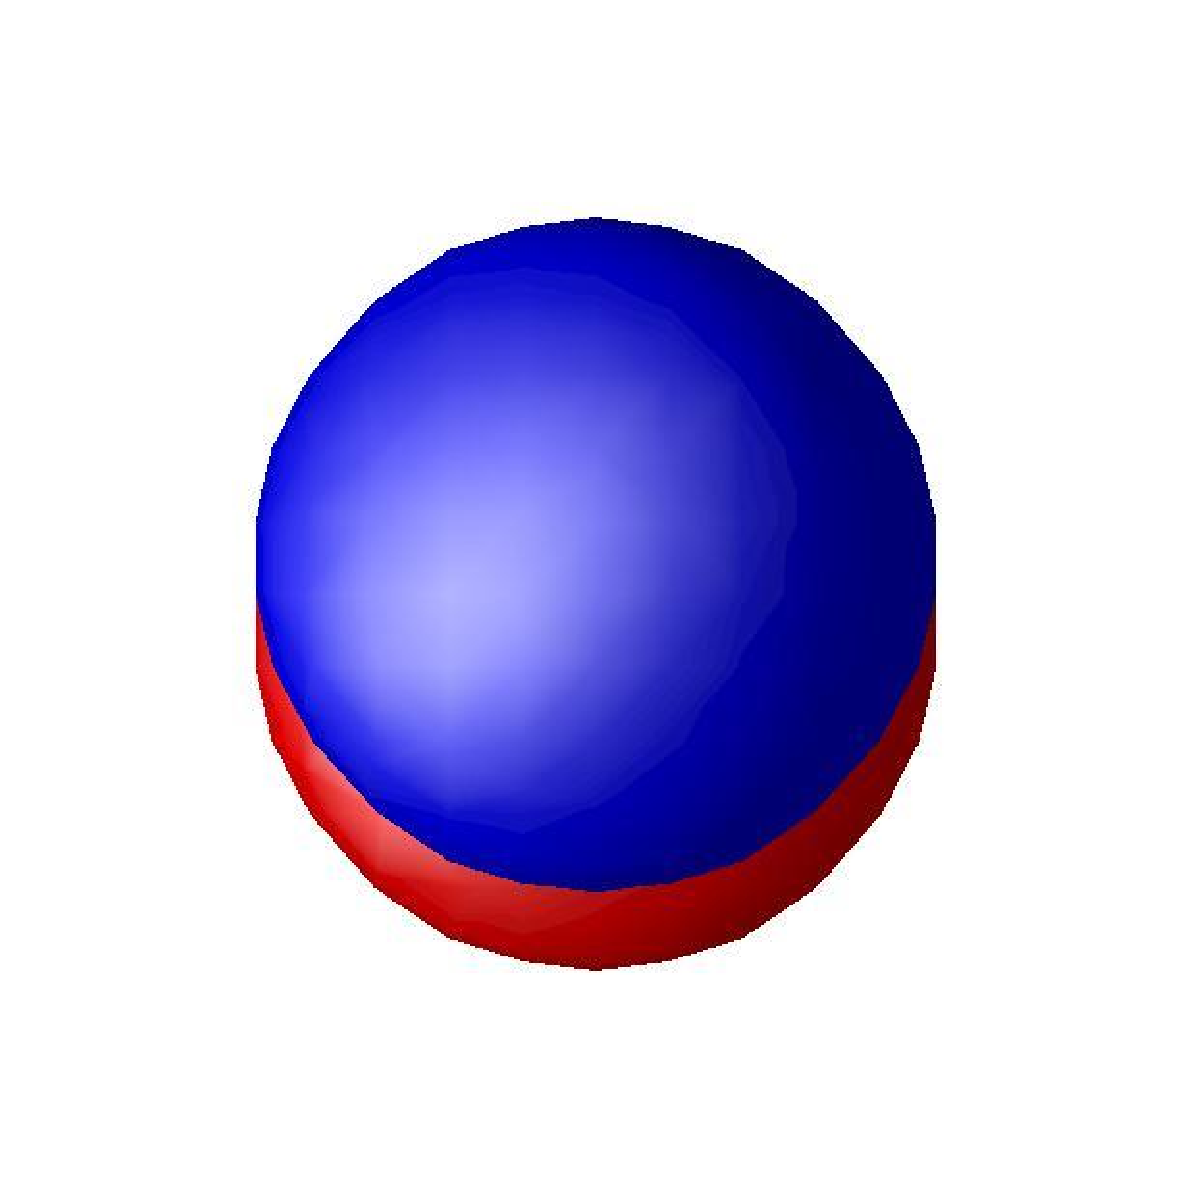
\includegraphics[width=0.3\unitlength]{img/pi02.eps}}
\put(0.32,0){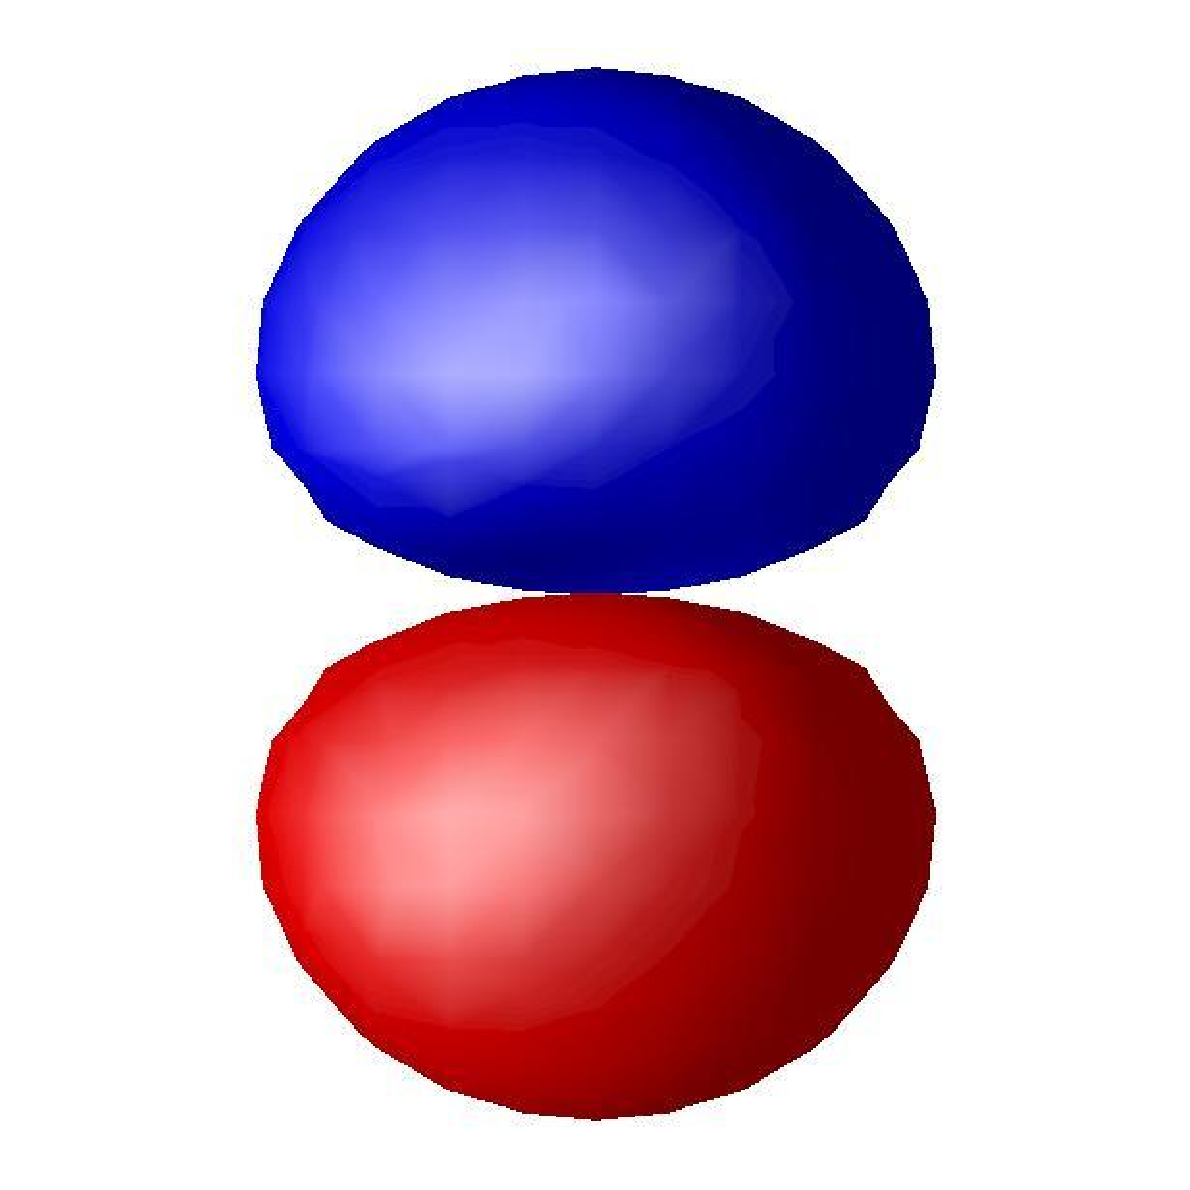
\includegraphics[width=0.3\unitlength]{img/pi03.eps}}
\put(0.64,0){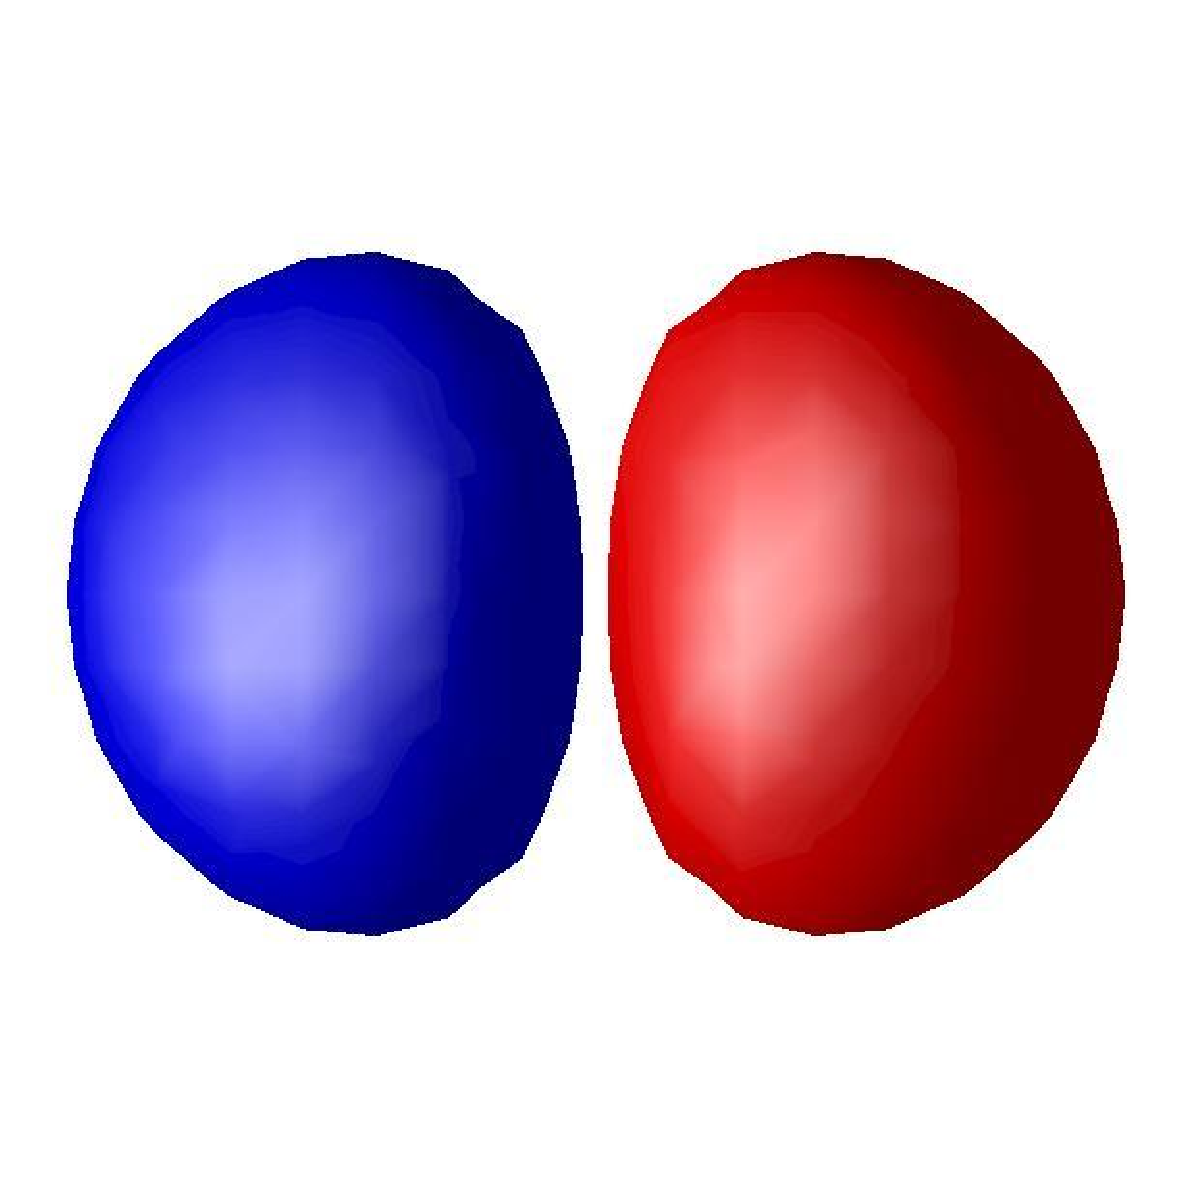
\includegraphics[width=0.3\unitlength]{img/pi04.eps}}
\end{picture}
\caption{
\label{figure:Nitrogen_pi_orbitals}
Second, third, and fourth KS orbitals of the Nitrogen atom,
showing the expected $p$ symmetry.
}
\end{figure}
\begin{sampleoutput}{The Nitrogen atom: The {\tt static/info} file}{output:info_file}
\begin{verbatim}
System name: system

Mesh:
  Type = sphere
  Radius  [A] =   5.000
  Spacing [A] = ( 0.180, 0.180, 0.180)    volume/point [A^3] =  0.00583
  # inner mesh =  89727
  Grid Cutoff [eV] =  1160.595

Exchange and correlation functionals:
      Exchange    : LDA  - non-relat.
      Correlation : LDA  - PZ81

SCF converged in    7 iterations

Eigenvalues [eV]
 #st   Eigenvalue    Occupation
   1   -18.378882       2.000000
   2    -7.248448       1.000000
   3    -7.248448       1.000000
   4    -7.248448       1.000000

Energy:
      Ion-ion     =      0.00000000
      Eigenvalues =    -58.50310712
      Potentials  =   -144.61568022
      Exchange    =    -51.46568858
      Correlation =     -7.28085027
      Total       =   -261.86532618

Dipole [A]:                    [Debye]
      <x1> =    6.19852E-17      2.97728E-16
      <x2> =    7.85171E-17      3.77134E-16
      <x3> =    1.15262E-16      5.53628E-16

Angular Momentum L [adimensional]
      L1 =    0.00000E+00
      L2 =    0.00000E+00
      L3 =    0.00000E+00

      L^2 =    5.99516E+00

Convergence:
      abs_dens = 2.57419616E-06 (1.00000000E-05)
      rel_dens = 5.14839231E-07 (0.00000000E+00)
      abs_ev = 1.98394791E-04 (0.00000000E+00) [eV]
      rel_ev = 9.22795382E-05 (0.00000000E+00)

Forces on the ions [eV/A]
 Ion                        x              y              z
   1         N       0.000000       0.000000       0.000000
\end{verbatim}
\end{sampleoutput}
The standard output is not the only file produced by octopus. After a ground-state
calculation, you should specially look at the the directory {\tt static}, that \octopus
will have created, placing on it a file called {\tt info}. The {\tt info}
file is displayed in the output files box number~\ref{output:info_file}. Some of its
contents are replicated in the standard output, already explained. The rest
of the information is, we hope, self-explanatory.

You will also notice the existence of a directory call {\tt tmp}. This is used by
the {\tt octopus} for internal uses, and for the moment we will not explain it here.

Also, a file called {\tt out.oct} shows up. It contains a list of all the variables
used in the run, either present in the input file or not. It is worthed to look at it
because it is the authorative way to know exactly what \octopus did -- the input
file may contain misspellings.

\subsection{Restarting}

Any ground-state calculation may be restarted later (to refine it if it did not
converge properly, or with any other purpose), provided that the contents of the {\tt tmp}
directory are preserved. You may try this now, changing in the input file the run
mode, which now should be set to:

{\tt CalculationMode = gs }

Also, please add the following three lines:
\begin{verbatim}
OutputWfs = yes
OutputWfsNumber = ``1-4''
OutputDX = yes
OutputAxisX = yes
OutputAxisY = yes
OutputAxisZ = yes
\end{verbatim}

You will now notice that the convergence procedure is closed in only
one iteration; the reason is that the starting point was now
the (already converged) output state of the previous run. This
is why the line {\tt Info: Loading rpsi.} is now output to
standard output.
\subsection{More output files, and visualization}
Now take a look at the {\tt static} directory. Besides the {\tt info}
file there are a bunch of new files, called {\tt wf-001-00x-1.dx},
and {\tt wf-001-00x-1.a=0,b=0}, where {\tt x} runs from 1 to 4 (the four
KS states), and where {\tt a} and {\tt b} are either {\tt x}, {\tt y} or {\tt z}.
Instructing the \octopus code to generate these files
was the task of the input variables that you just added.
These files contain various functions related to the system (in this
case, wavefunctions) for their visualization.
\begin{mylist}
\item {\tt OutputWfs = yes}\\
This variable asks \octopus to print the wavefunctions. One may also wish
to print densities, potentials, etc. In the manual you may find the corresponding
input variables ({\tt OutputDensity}, etc).
\item {\tt OUtputWfsNumber = '1=4'}\\
This variable specifies which wavefunctions to print: {\tt '1-4'} asks
for the KS orbitasl running from one to four; {\tt '1,2,7-10'} would
ask for the first two, and the ones from seven to ten.
\item {\tt OutputDX = yes}\\
This variable forces the code to print the functions in the format
native to the OpenDX program. This program permits ``sophisticated'' data
visualization (isosurfaces, contour plots, etc).

The Appendix A introduces the use of the utilities included along with \octopus
to facilitate the visualization with OpenDX. In Figure~\ref{figure:Nitrogen_pi_orbitals}
you may see isosurfaces of the obtained $p_x$, $p_y$ and $p_z$ Kohn-Sham orbitals of Nitrogen.

\item {\tt OutputAxisX/Y/Z = yes}\\
This variable is the responsible for the appearance of the files {\tt wf-001-00x.x=0,y=0},
{\tt wf-001-000x.x=0,z=0} and {\tt wf-001-000x.y=0,z=0}. These files contain the values of
the wavefunctions along the $z$, $y$ and $x$, respectively, in the format
coordinate, real value and imaginary value. This way you can plot the functions
with easier-to-use plotting programs.

\end{mylist}

\subsection{Finding a good spacing for the Nitrogen pseudopotential}

\begin{floatingfigure}{0.5\textwidth}
\includegraphics[width=0.48\textwidth]{img/spacing.eps}
\caption{Convergence of the total energy, and of $s$ and $p$ eigenvalues of
the Nitrogen atom, with respect to the grid spacing.
\label{figure:convergence_study}
}
\end{floatingfigure}
The key paramenter of a real-space calculation is the spacing between the points
of the mesh. In the current version of \octopus, the grid is regular, so there is
only one grid spacing.\footnote{
In fact, if you use the {\tt parallelepiped} shape for your simulation box, you may
define different spacings in each direction, by using the {\tt \%spacing} block, instead
of the {\tt spacing} variable.
}
The first step in any calculation should then be making sure that this spacing is
good enough for our purposes. This should be done through a convergence study, very
similar to the ones performed in plane-wave calculations.

The needed spacing essentially depends on the pseudopotentials that are being
used. The idea is to repeat a series of ground-state calculations, with identical input files
except for the grid spacing. One convenient way to do it is by commenting
out the line {\tt spacing = 0.18} line in the previous input file (comments
are initiated with the {\tt \#} character). Then one can use the little script
presented in the input file~\ref{input:script_convergence}.

After the runs, you may then analyze the {\tt info} files, and plot, for example,
the eigenvalues or the total energy versus the grid spacing. The results, for this
particular example, are shown in Figure~\ref{figure:convergence_study}. A rather good spacing
for this Nitrogen pseudopotential seems to be 0.18\AA; probably a larger one may also
be used without compromising the results.


\begin{sampleinput}{Sample script for a convergence study}{input:script_convergence}
\begin{verbatim}
#! /bin/bash

list=''0.26 0.24 0.22 0.20 0.18 0.16 0.14''

for i in ${list}
do

test -d ${i} || mkdir ${i}

cd ${i}
cp ../inp ../N.xyz .

echo ``spacing=${i}'' >> inp
echo -n ``Launching octopus for spacing=${i}...''
octopus < inp > out 2>&1 err
echo `` Done.''

rm -rf tmp

cd ..

done
\end{verbatim}
\end{sampleinput}


\section{Another example: the Nitrogen molecule}
A small step forward is performing calculations for the Nitrogen molecule. Some small
modifications to our previous input file for the Nitrogen atom allows us to calculate
the dimer. Note that now we do not need the {\tt \%Occupations} block, and that in this
case we do not make use of any external XYZ file -- the geometry is described internally
in the input file via a {\tt \%Coordinates} block. In this way we can make sure of the
user defined variable {\tt N2\_bondlength}. Also, we have used a couple of more variables
to refine the SCF performance ({\tt EigensolverInitTolerance}, {\tt EigenSolverFinalTolerance}
and {\tt EigenSolverFinalToleranceIteration} (you may want to check the manual
to understand their meaning).
This input file should lead to a total pseudoenergy of -541.54~eV. And, noticeably, there exists
an attractive force between the atoms of 0.81~eV/\AA: The experimental equilibrium geometry
is obviously not the equilibrium geometry in the LDA approximation.
\begin{sampleinput}{One simple input file for a Nitrogen molecule}{input:nitrogen_molecule}
\begin{verbatim}
CalculationMode = gs_start

units = 'eVA'

Nitrogen_mass = 14.0
Nitrogen_z = 7
N2_bondlength = 1.098

%Species
'N' | Nitrogen_mass | Nitrogen_z | 'tm2' | 1 | 0
%

%Coordinates
'N' | -N2_bondlength/2 | 0 | 0 | no
'N' |  N2_bondlength/2 | 0 | 0 | no
%

BoxShape = sphere
radius = 5.0
spacing = 0.18

LocalPotentialSpace = real_space

EigenSolverInitTolerance = 1.0e-4
EigenSolverFinalTolerance = 1.0e-7
EigenSolverFinalToleranceIteration = 5

TypeOfMixing = broyden
\end{verbatim}
\end{sampleinput}

\begin{exerciselist}
\item You may investigate the effects of the different SCF related variables
({\tt EigenSolverFinalTolerance}, {\tt TypeOfMixing}, etc), and their
different values, which you may find in the manual.
\end{exerciselist}

\subsection{The other convergence study: the box size}

The grid spacing is not the only parameter whose convergence one should check
carefully when doing the ground-state calculation of a system in real-space. Also,
one should make sure that the system does not ``see'' the borders of the simulation
box, so that the imposed zero boundary conditions are consistent -- in other words,
that the box is sufficiently large.

\begin{exerciselist}
\item Commenting the input line {\tt radius = 5.0} in input file~\ref{input:nitrogen_molecule},
and building a similar script to the input file~\ref{input:script_convergence}, you may do a convergence
study of a Nitrogen molecule with respect to the radius of the sphere that is used as the
simulation box.
\end{exerciselist}

\subsection{The equilibrium geometry in LDA/GGA}

\begin{floatingfigure}{0.5\textwidth}
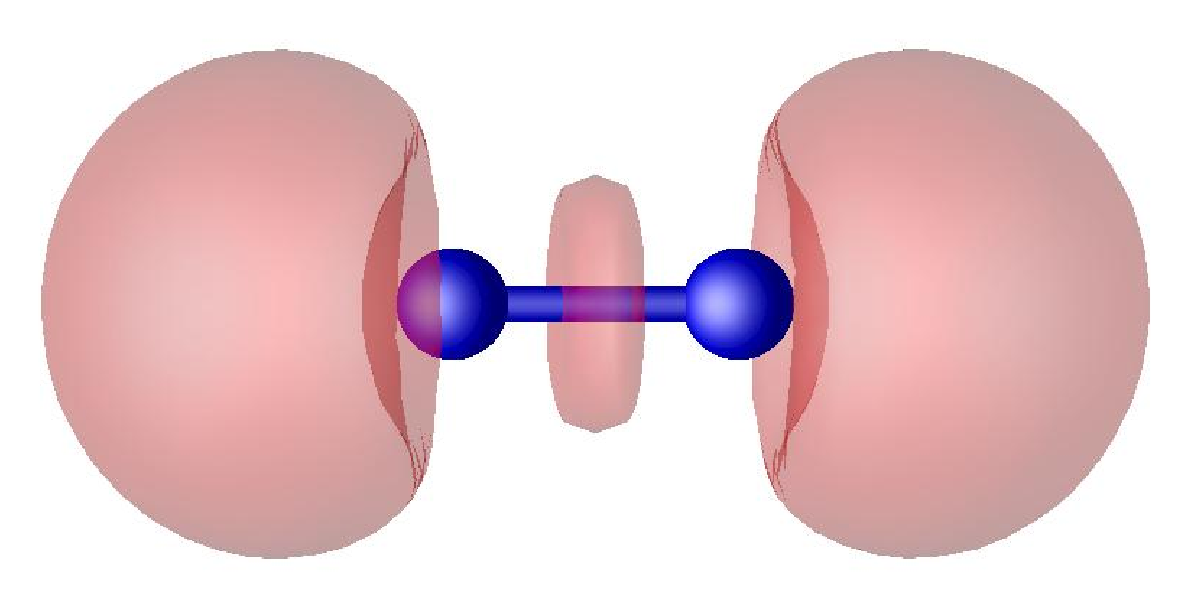
\includegraphics[width=0.48\textwidth]{img/elf.eps}
\caption{ELF of the Nitrogen molecule
\label{figure:elf_N2}
}
\end{floatingfigure}
Unfortunately, in version 1.4 we did not implement a proper minimization
algorithm to find equilibrium geometries. This deficiency will be properly
solved in future version 2.0. In any case, for the dimer, with only one degree of
freedom we can properly find the (wrong) equilibrium bond-length of the Nitrogen molecule.
Once again, make use of input file~\ref{input:nitrogen_molecule}, but this time
commenting out the line {\tt N2\_bondlength = 1.098}. Then one can define a script,
such as the in input file~\ref{input:script_dimer_bondlength}, to calculate the
total pseudo-energy as a function of the bond length, thus permitting us to 
obtain the equilibrium geometry in the minimum of the curve. Note that you may want
to add more points to the {\tt list} variable, in order to refine the curve. In
any case, we have obtained an equilibrium geometry of 1.092~\AA, where the interatomic
force is of only 0.034~eV/\AA~(note that one atomic unit of force is 51 times larger
than 1~eV/\AA).

It is tempting to analyze the Kohn-Sham states in the same manner than quantum-chemists
do for the Hartree-Fock orbitals. This tutorial is not the place to comment on such
practices, but we would like to draw the attention towards the electron localization
function (ELF), a function crafted to help to visualize bonds. In Fig.~\ref{figure:elf_N2}
you may see one isosurface of the ELF that we have obtained, at the equilibrium geometry.\footnote{
To get a nicer and smoother picture, we have used 0.14\AA of grid spacing.
}
You may see the triple bond between the two Nitrogen atom, along with two Hydrogen pairs
at the sides of each atom. This plot may be obtained by making use of the
{\tt OutputELF = yes} option in the input file, along with the {\tt OutputDX} variable.


\begin{sampleinput}
{Script to obtain the energy curve of the Nitrogen dimer in the LDA approximation}
{input:script_dimer_bondlength}
\begin{verbatim}
#! /bin/bash
list="0.98 1.00 1.02 1.04 1.06 1.08 1.10 1.12 1.14"

for i in ${list}
do

test -d ${i} || mkdir ${i}
cd ${i}

cp ../inp .
echo "N2_bondlength=${i}" >> inp
echo -n "Launching octopus for bondlength=${i}..."
octopus < inp > out 2>&1 err
echo " Done."

rm -rf tmp

cd ..
done
\end{verbatim}
\end{sampleinput}

\begin{exerciselist}
\item You may want to check how good the LDA vibrational frequency is; it can 
be readily calculated out of the energy curve that you have just calculated.
\end{exerciselist}

\section{One time-dependent run}

OK, it is about time to do TDDFT (up to now only ground state DFT was used).
Let us perform a calculation of the time evolution of the density of the
Nitrogen molecule. The reason to do ground state DFT is that for any time-dependent
calculation you will need first to do a ground-state calculation. You may
start from the calculation that you have just done (Input file~\ref{input:nitrogen_molecule}).
Once that you have a proper ground-state (stored in the {\tt tmp} directory,
you should switch on a new run mode, {\tt CalculationMode = td\_start}, and
add a few more variables to the input file:
\begin{verbatim}
T=0.1
dt = 0.002
TDEvolutionMethod = aetrs
TDMaximumIter = T/dt
TDTimeStep = dt
\end{verbatim}
If you run the \octopus once again, it will run for a few minutes, depending
on the speed of your machine. The most relevant chuncks of the standard output
are shown in the Output box~\ref{output:td_sample1}.

\begin{sampleoutput}{Time-evolution of the Nitrogen molecule}{output:td_sample1}
\begin{verbatim}
Info: Setting up TD.
Info: Evolution method:  Approx.Enforced Time-Reversal Symmetry
Info: Exponential method: 4th order expansion.
Info: Initializing zpsi.
Info: Time-dependent simulation.
  Iter           Time        Energy     Elapsed Time
      1       0.002000   -541.542073         4.800
      2       0.004000   -541.542073         4.560
      3       0.006000   -541.542073         3.880
...
     48       0.096000   -541.542073         7.420
     49       0.098000   -541.542073         7.620
     50       0.100000   -541.542073         7.490
Info: Cleaning up occupational analysis.
Info: Cleaning up TD.
Info: FFT deallocated from slot    1
Info: Calculation ended on 2005/02/01 at 16:33:28
\end{verbatim}
\end{sampleoutput}
It is worthwhile to comment a few things:
\begin{mylist}
\item We have just performed the time-evolution of the system, departing from
the ground-state, under the influece of no external perturbation. As a consequence,
the electronic system does not evolve. The total energy does not observe (this you
may already see in the output file, the third column of numbers), nor should
change any other observable. Thus this kind of runs are only useful to check that
the parameters that define the time evolution are correct.
\item As the evolution is performed, the code probes some observables and prints
them out. These are placed in some files under the directory {\tt td.general}, which
should show up in the working directory. In this case, only one file will show
up, the {\tt multipoles} file. This file contains a large number of columns of data. Each
line corresponds with one of the time steps of the evolution (except for the first
three lines, that start with a {\tt \#} symbol, and which inform about the
meaning of the numbers contained in each column, and their units). A brief overview
of the information contained in this file follows:
\begin{list}{o}
{
\setlength{\parskip}{0pt}
\setlength{\topsep}{0pt}
\setlength{\partopsep}{0pt}
\setlength{\itemsep}{0pt}
\setlength{\parsep}{0pt}
}
\item The first column is just the iteration number.
\item The second column is the time.
\item The third column is the dipole moment of the electronic system, along the $x$ direction:
\begin{equation}\nonumber
\langle \Phi (t) \vert \hat{x} \vert \Phi(t)\rangle = 
\int\!\!{\rm d}^3\!\!r\; x\,n({\bf r})~\,.
\end{equation}
Later columns show general electronic moments; the reason for singling out this specific
dipole here is explained later.
\item Next three columns (headed {\tt n.dip.(1)}, {\tt n.dip.(2)} and {\tt n.dip.(3)}) represent
the dipole moment of the nuclei along the $x$, $y$ and $z$ directions. Of course, in the particular
run that we just did these are null all the time.
\item The following columns present the multipoles of the system:
\begin{equation}\nonumber
\langle \Phi (t) \vert \hat{M}_{lm} \vert \Phi(t)\rangle = 
\int\!\!{\rm d}^3\!\!r\; r^lY_{lm}({\bf r})\,n({\bf r})~\,.
\end{equation}
The index $l$ runs, in this case, from zero to one, but higuer order moments may
be printed by making use of the input variable {\tt TDDipoleMax}.

Note that the first multipole is the monopole: $(l,m)=(0,0)$ -- i.e. the charge, except
for a $\frac{1}{4\pi}$ factor.
\end{list}

\item The meaning of the three new variable that we have introduced
in the input file is rather obvious: {\tt TDEvolutionMethod} to establish which
algorithm must approximate the evolution operator; {\tt TDMaximuIter} to tell
the code how may time steps to perform; and {\tt TDTimeStep} to fix
the length of each time step. And note that, for convenience, we have previously
defined a couple of variables, {\tt T} and {\tt dt}. We have made use of one of
the possible propagators, {\tt aetrs}. The manual explains about the possible
options; in practice this choice is usually good.
\end{mylist}


\subsection{Another important parameter: the time step}


A key parameter is, of course, the time step. Before making long-scale calculations,
it is worthwhile spending some time choosing the largest time-step possible. This
time-step depends crucially on the system under consideration, on the applied perturbation,
and on the algorithm chosen to approximate the evolution operator. Also, there is
another input variable that was not employed, relying on its default value,
{\tt TDExponentialMethod}. Since most propagators rely on algorithms to calculate
the action of the exponential of the Hamiltonian, one can specify which algorithm
can be used for this purpose.
\begin{exerciselist}
\item You may want to learn about the possible options that may take {\tt TDExponentialMethod},
and {\tt TDEvolutionMethod} -- take a look at the manual.
\item Fixing the propagator algorithm (for example, to the default value), 
investigate how the several exponentiation methods work (for example, the three
polynomial schemes: standard, Chebychev and Lanczos). This means finding out what
maximum time-step one can use without compromising the proper evolution.
\item And fixing now the {\tt TDExponentialMethod}, one can now play around with
the various propagators (note that the ones based on the split-operator idea do not
rely on any exponential method but their own).
\end{exerciselist}

\subsection{Optical response}


\subsection{Adding a laser field, and response to high fields}

Now we will add a time-dependent external perturbation to the molecular
Hamiltonian. Add the lines in Input file~\ref{input:laser} to the previous
input file.
\begin{sampleinput}{Parameters that describe a laser field}{input:laser}
\begin{verbatim}
envelope = 2
w = 5.0
cycles = 4
tau = (pi/w)*cycles
t0 = tau
%TDLasers
1 | 0 | 0 | intensity | frequency | envelope | tau | t0
%
\end{verbatim}
\end{sampleinput}
The only real \octopus variable is the {\tt \%TDLasers} block. However, instead of
placing the numbers there it is handier to define them as user defined variables,
as we have done previously. You should carefully read the manual page dedicated
to the laser fields: the particular laser pulse that we have employed is the one
whose envelope function is a cosine (the option 2 in the block sixth entry of the
block, which is entered through the user defined variable {\tt envelope}).

\begin{figure}
\centerline{
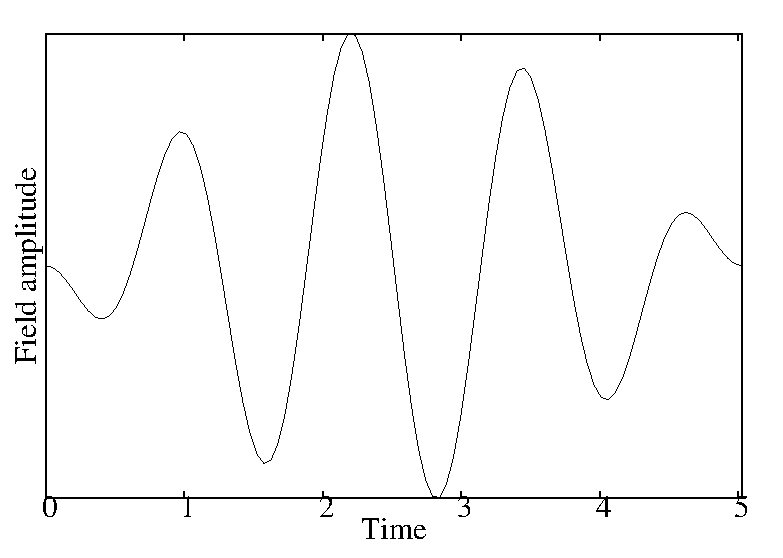
\includegraphics[width=0.4\textwidth]{img/laser.eps}}
\caption{Field amplitude of the laser field imposed in Input file~\ref{input:laser},
\label{figure:laser}
}
\end{figure}

As you notice, this defines a laser with only four cycles (this is set by the
user defined variable {\tt cycles}. Of course you could directly set the duration
{\tt tau} directly, but this is an illustration of how the user defined variables
may be useful.

Now you are ready to setup a run with a laser field. Be careful to set a total time
of propagation able to accomodate the laser shot, or even more if you want to see
what happens afterwards. You may also want to consult the meaning
of the variables {\tt TDOutputLaser} and {\tt TDOutputEnergy}.

A couple of important comments:
\begin{mylist}
\item You may supply several laser pulses: simply adding more lines
to the {\tt TDLasers} block.
\item When an external field is present, one may expect that unbound
states may be excited, leading to ionization. In the calculations, this
is reflected by density reaching the borders of the box. In these cases,
the proper way to proceed is to setup absorbing boundaries (variables
{\tt AbsorbingBoundaries}, {\tt AbWidth} and {\tt AbHeight}).
\end{mylist}




\section{Molecular Dynamics}

\section{Excited states in linear response theory}


%%%%%%%%%%%%%%%%%%%%%%%%%%%%%%%%%%%%%%%%%%%%%%%%%%%%%%%%%%%%%%%%%%%%%%%%%%%%%%%
\section{Model potentials}
%%%%%%%%%%%%%%%%%%%%%%%%%%%%%%%%%%%%%%%%%%%%%%%%%%%%%%%%%%%%%%%%%%%%%%%%%%%%%%%

\subsection{Harmonic oscillators, and quantum dots}

\octopus permits to do one or two-dimensional calculations.

\subsection{A one-dimensional model for the Helium atom}

The next example is a one-dimensional model of the Helium atom. The calculation
in this case is not a DFT one, but an exact solution of the Schr{\"{o}}dinger
equation -- not an exact solution of the Helium atom, however, since it is a
one-dimensional model. Calling $x$ and $y$ the coordinates of the two electrons,
the Hamiltonian would be:\footnote{
Note that the usual Coulomb interaction between particles is usually substituted,
in 1D models, by the {\em soft Coulomb} potential, $u(x)=(1+x^2)^{(-1/2)}$
}
\begin{equation}
\hat{H} = -\frac{1}{2}\frac{\partial^2}{\partial x^2}
          -\frac{1}{2}\frac{\partial^2}{\partial y^2}    
+\frac{-2}{\sqrt{1+x^2}}+\frac{-2}{\sqrt{1+y^2}}+\frac{1}{\sqrt{1+(x-y)^2}}.
\end{equation}
Instead of describing two
electrons in one dimension, however, we may very well think of one electron in two dimensions,
subject to a external potential with precisely the shape given by previous equation. 
Since the Hamiltonian is idential, we will get the same result.
Whether we regard $x$ and
$y$ as the coordinates of two different particles in one dimension or as the
coordinates of the same particle along the two axes in two dimensions is
entirely up to us. Since it is usually easier to treat only one particle, we
will solve the one-dimensional Helium atom in two dimensions.
We will also get a two dimensional wave-function. In order to plot this
wave-function we specify an output plane instead of an axis. A possible
input file is given in Input File~\ref{input:laser}.

\begin{sampleinput}{The 1D-model of the Helium atom}{input:laser}
\begin{verbatim}
SystemName="He"
CalculationMode = gs_start
Dimensions=2
NonInteractingElectrons = yes
radius = 10
spacing = 0.1
OutputWfs = yes
OutoutPlaneZ = yes
%Species
"He" | 4 | 1 | "-2/(1+x^2)^(1/2)-2/(1+y^2)^(1/2)+1/(1+(x-y)^2)^(1/2)"
%
%Coordinates
"He" | 0 | 0 | 0 | no
%
\end{verbatim}
\end{sampleinput}






\appendix

\section{Visualization with OpenDX}

\end{document}